%%%%%%%%%%%%%%%%%%%%%%%%%%%%%%%%%%%%%%%%%%%%%%%%%%%%%%%%%%%%%%%%%%%%%%%%%%%%%%%%
%%% Background
%%%%%%%%%%%%%%%%%%%%%%%%%%%%%%%%%%%%%%%%%%%%%%%%%%%%%%%%%%%%%%%%%%%%%%%%%%%%%%%%

%% In a thesis, every section starts a new page, hence \clearpage
\clearpage
\section{Background and related work}
\label{sec:background}

\subsection{Process mining}

Process mining starts from the concept of an \emph{event log}.
An event log is a collection of recorded data for an information system.
Activities executed in the system leave records which are stored in the event log.
\emph{Process mining} describes methods of using the event log data to extract useful information.
The information can be used to discover processes without prior knowledge, to find bottlenecks and inefficiencies, to detect and understand anomalies, and to support redesign actions \cite{van2015extracting}.
In this thesis I look at \emph{process discovery}, which means finding the underlying process model
by reading the event log.
In process discovery the model should be generated without any a-priori information, meaning that the algorithm should be unsupervised \cite{van2013discovering}.
The process model can be expressed as a directed graph or a \emph{Petri net}.
These models can be used for business intelligence (BI) solutions, or they can be compared to the real life
known models to check conformance \cite{van2013discovering}.


Discovering strictly sequential processes from event logs is straightforward. However, modern systems are increasingly concurrent which complicates the issue. 
Parallel systems generate events in an undetermined order based on how the processes are interleaved. 
When the events are logged the order is realized resulting in a totally ordered sequential log \cite{van2004workflow}. 
The challenge is having to discover and construct the parallelism from the event log.
Furthermore, the event log may be \emph{incomplete}, which means not all possible behaviour is present in the logs \cite{van2013discovering}.
Additionally, the event logs can be \emph{noisy} and contain random infrequent behaviour \cite{van2013discovering}.
It may be undesirable to present the infrequent behaviour in the models.
These characteristics give the task of process discovery challenging trade-offs.

\subsubsection{Event logs and traces}

\label{sec:eventtheory}

\begin{definition}
Let $A$ be the set of all \emph{events}. 
$\sigma \in A^*$ is a \emph{trace} describing a sequence of events.
The event log $L \in \mathbb{B}(A^*)$ is a \emph{multi-set} of \emph{traces}.
\end{definition}

A process consists of a set of distinct \emph{activities}.
An activity is a well-defined step belonging to the process (for example, ''resize an image'').
Each event in the event log is a log entry documenting an execution of an activity.
In other words, $A$ is the vocabulary of events.
The event may also hold additional information about the process.
A workflow \emph{trace} contains a sequence of events documenting a single execution of the process (a \emph{process instance}).
This kind of single process execution is called a \emph{case} (later in this thesis also: \emph{submission}).
The event log can be seen as a \emph{multi-set} of \emph{traces}. 
A multi-set (a \emph{bag}) is a set that allows multiple instances of the set's elements. \cite{van2015extracting}

In this thesis it is assumed that any concurrent execution of events can be recorded into
an ordered and sequential event log. 
The concurrent execution generates randomly ordered sequences.
The parallelisms can be discovered by observing the different traces and their frequencies.
For example, for a process consisting of activities $a,b,c,d,e \in A$, one trace could be 
$\langle a,b,c,d,e \rangle$ and another $\langle a,c,d,b,e \rangle$.
These different traces could be found in the event log a number of times, some more frequent than others.
In process discovery the task is to construct a model with sequential and parallel steps 
that describes a process that can generate these traces \cite{van2013discovering}.
The frequency of a trace matters in process discovery, and this is why the event log is a multi-set.
Figure \ref{fig:tracevslog} illustrates the difference of the mathematical abstraction of a multi-set of traces in a) and a real-life event log with interleaved traces in a physical log file.

\begin{figure}[htb]
\centering 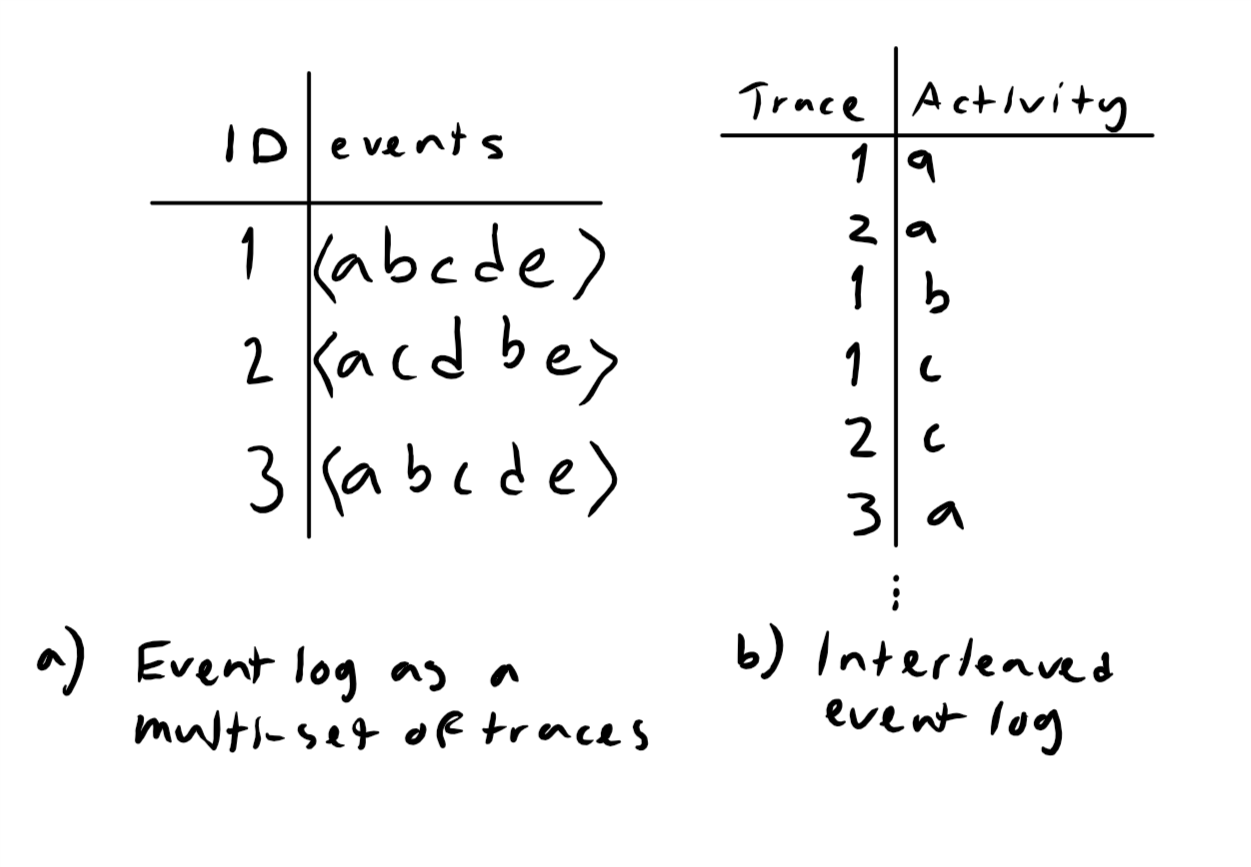
\includegraphics[width=0.7\linewidth]{gfx/figures/traceeventlog.png}
\caption{Event logs illustrated \nyi{id-trace, trace ID-event} \nyi{fix n.2}}
\label{fig:tracevslog}
\end{figure}

When dealing with discovering processes from event logs, there are two clear challenges: \emph{incompleteness} and \emph{noise}. 
Discovering the model from the event log is difficult since one cannot assume that all the possible traces are present \cite{van2013discovering}. 
This is because the order how parallel processes interleave is random. 
For a set of $n$ concurrent processes, there are $n!$ possible interleavings.
The number of sequences observed in the logs \cite{van2007business} is often much smaller than the number of all possible sequences.
Moreover, some sequences can be inherently more infrequent that others. 
Such behaviour can be seen as undesirable noise, but sometimes infrequent traces may also present important information.
This leads to the need of making decisions about trade-offs. 
The model should describe the process accurately, even when the event log is incomplete or noisy.

Van der Aalst et al. \cite{van2013discovering} describe four criteria that need to be balanced when generating a model from a log: fitness, precision, generalization, and simplicity.
\emph{Fitness} measures whether the model fits the log, meaning that the traces in the event log can be generated by the discovered model.
\emph{Precision} measures whether the model allows only the behaviour observed in the event log. The model should describe the traces in the log but should not allow completely unrelated behaviour not seen in the traces.
\emph{Generalization} relates to the unseen behaviour. The model should be general enough that it describes the process while allowing the cases that were not observed in the specific set of sequences.
Lastly, \emph{simplicity} relates to the noisiness. The models should be as simple as possible and undesirable rare or exceptional behaviour should not be included if it increases the model complexity.


\subsubsection{Process models and discovery}
\label{sec:processmodelsdsc}

A simple way to describe a process model is a \emph{directed graph}. A directed graph is a set of \emph{nodes} that are connected together by \emph{edges}. 

\begin{definition}
A directed graph $G = (\mathcal{N}, \mathcal{E})$ consists of the set $\mathcal{N}$ of nodes and the set $\mathcal{E} \subseteq \{ (x,y) | x,y \in \mathcal{N} \} $ of edges, which are ordered pairs of nodes.
\end{definition}

A process can be described as a directed graph by having a graph node for each activity of the process ($\mathcal{N} = A$). The graph edges describe the possible transitions between the activities.
In this model, any two parallel activities $a, b \in A$ will have directed arcs $(a,b)$ and $(b,a)$ between them.
A log is generated by traversing through the graph and visiting all nodes \textit{exactly once}.
Figure \ref{fig:directedgraph} illustrates an example of a directed graph.
The graph shown has two nodes $c$ and $d$ which are parallel.
By following the directed arcs and visiting each node exactly once, the graph shown can generate exactly two distinct traces: $\langle a,b,c,d,e \rangle$ and $\langle a,b,d,c,e \rangle$.
\nyi{cite a formal definition}

\begin{figure}[htb]
\centering 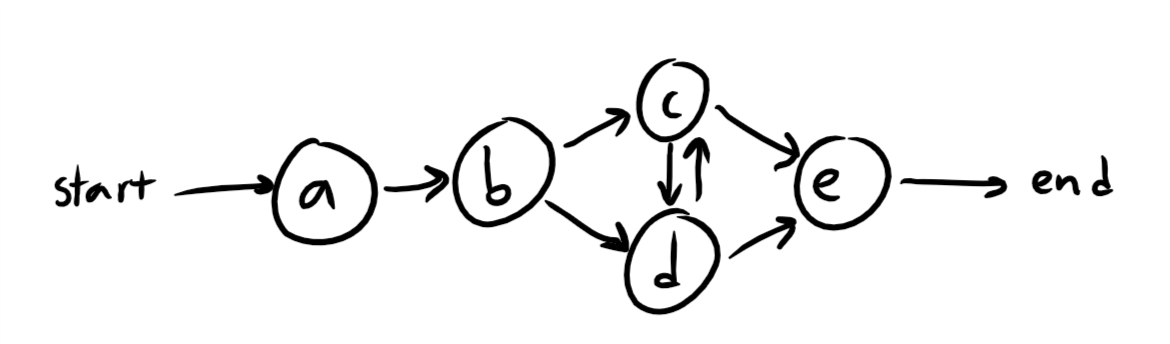
\includegraphics[width=0.7\linewidth]{gfx/figures/directedgraph.png}
\caption{An example of a directed graph}
\label{fig:directedgraph}
\end{figure}

A \emph{Petri net} \cite{rozenberg1998lectures} can be used as a more detailed process model. A Petri net consists of \emph{places}, \emph{transitions}, and directed arcs connecting them. In this thesis I focus on \emph{finite nets} where the sets forming a Petri net are finite.

\begin{definition}
A Petri net is a tuple $N = (S, T, F)$ which consists of:
\begin{enumerate}
    \item a set $S$ of \emph{places},
    \item a set $T$ of \emph{transitions} in a way that $S \cap T = \emptyset$
    \item a set $F$ (flow relation) of directed arcs: $F \subseteq (S \times T) \cup (T \times S)$ 
\end{enumerate}
\end{definition}

In a Petri net, the places and transitions $S \cup T$ are called the \emph{elements} of $N$.
For any element $x \in S \cup T$ its \emph{pre-set} ${}^\bullet x$ is all the elements that have a directed arc to $x$, that is ${}^\bullet x = \{y \in S \cup T | (y,x) \in F\}$. Similarly its \emph{post-set} $x^\bullet$ is defined as 
$x^\bullet = \{y \in S \cup T | (x,y) \in F\}$.
A Petri net can be mapped to a directed graph by creating equivalent nodes for each place and directed edges for each transition.

Van der Aalst et al. \cite{van2013discovering} use a subclass of Petri nets called a \emph{workflow net} to describe processes. A workflow net (WF-net) is a Petri net with some further restrictions, to make it more suited for process discovery. In their description, a WF-net needs a single starting point (an input place) and a single ending point (an output place). Furthermore they define that a WF-net needs to be \emph{strongly connected}, meaning every node is on a path from the start to the end.

\begin{definition}
Let $N = (S, T, F)$ be a Petri net. $N$ is a workflow net \emph{iff}:
\begin{enumerate}
    \item $S$ contains an input place $i$ such that ${}^\bullet i = \emptyset$ (starting point)
    \item $S$ contains an output place $o$ such that $o^\bullet = \emptyset$ (ending point)
    \item \nyi{Formulate this formally} (connectedness)
\end{enumerate}
\end{definition}

With the definitions for event logs, traces and WF-nets, we can describe \textbf{process discovery} as an algorithm that maps any event log $L$ into a model such as a directed graph or a Petri net that describes the underlying process that generated the event log.

\subsubsection{\textalpha-algorithm}
\label{sec:alphaalgorithm}
Constructing concurrent process models from an ordered event log is a challenging task.
The event log is a linear and ordered list of events.
The log does not directly express the dependencies between the events.
To find the dependencies and thus the shape of the process model, it needs to be extracted with an algorithm.

The \textalpha-algorithm is a process discovery algorithm that reads ordered event logs.
The algorithm discovers parallelism by comparing the order of events in different traces.
In a trace, the activities that depend on another activity always come later in the trace.
However, the activities that are parallel and have no such dependency can come in any order regarding each other.
Thus, in different traces the parallel activities are ordered differently. 
This is the main idea behind the \textalpha-algorithm.

A detailed mathematical description of the \textalpha-algorithm can be found in \cite{van2004workflow}.
The idea of the algorithm is:

\begin{enumerate}
    \item Find all the events that appear in event log $L$. I call this the \emph{vocabulary}. This corresponds to all the transitions $T_L$ in the WF-net.
    \item Find all the events that appear as the first event in any trace (the \emph{start transitions}).
    \item Find all the events that appear as the last event in any trace (the \emph{end transitions}).
    \item Find all pairs of sets of events $(A,B)$ that have a (causal) dependency in all the traces. This means that all events in $A$ always come before all the events in $B$ in all the traces.
    \item Reduce the set of pairs discovered in the previous step to only include the ''maximal pairs'' (see below). 
    \item Create a place for each pair $(A,B)$ from the previous step. Additionally, create places for a starting point $i$ and an ending point $o$. This will be the set of places $S_L$.
    \item Connect the arcs (the flow relation $F_L$). All start transitions from step 2 will have $i$ as their input place and all end transitions from step 3 will have $o$ as their output place. All the places for each pair $(A,B)$ will have transitions in $A$ as their input node and transitions in $B$ as their output node.
    \item The result is a WF-net $\alpha(L) = ( S_L, T_L, F_L )$.
\end{enumerate}

In step 5, the set of ''maximal pairs'' means that there are no pairs which include subsets of another pair. For example, the pairs $\{(\{a\},\{b,c\}),(\{a\},\{b\}),(\{a\},\{c\})\}$ can be reduced into just $\{(\{a\},\{b,c\})\}$.

In essence, the \textalpha-algorithm tries to find arcs that form a WF-net describing the causal dependencies observed over all the traces in the event log. 
For example, if activity $b$ comes after activity $a$ in all the traces, then it suggests a causal dependency $a \rightarrow b$.
On the other hand, if in some traces $a$ comes after $b$ and some others before, then it suggests that the activities do not depend on each other and are parallel.

There are some limitations to this algorithm.
The \textalpha-algorithm assumes that the event log is complete and has accurate ordering \cite{van2013discovering}. This means that all the events are present in the logs, and that the time-ordering in the traces corresponds to causal relations accurately. Furthermore, there can be different WF-nets that create similar traces \cite{van2013discovering}. In other words, different process models can create the same traces.
The algorithm is also not suited to dealing with non-local dependencies \cite{van2013discovering}.
For example, if $a \rightarrow b$, $b \rightarrow c$, and $a \rightarrow c$, this $a \rightarrow c$ dependency is said to be ''non-local'', since from the logs it would only appear that $b \rightarrow c$. 

% ################################

\subsection{Machine learning}

Machine learning means the study and development of algorithms that give computers the ability to learn from data without being explicitly programmed for that data. 
The traditional approach in programming is to explicitly define the steps the computer should take to solve a problem.
However, sometimes you know the input to a problem and what the solution should be, but not how to get to the solution.
Figure \ref{fig:traditionalvsml} illustrates this fundamental difference.
For example, we could have a thousand photos of birds and a thousand photos of animals other than birds.
For these photos we know exactly which ones are the birds, but we don't know exactly what rules in the pixels of an image makes it a bird photo.
This situation is what machine learning algorithms are meant for.

Machine learning is data driven and the focus is less on traditional programming instructions.
The machine learning algorithms focus on finding patterns and models in data.
The patterns can then be used to process new data or make predictions.

Supervised learning is a subset of machine learning. In supervised learning, the input for the computer is a set of \textit{training data} with predefined labels. 
This training data is the ''known'' data points of the ''seen'' data.
For example in the case of email spam detection, the training data could be a set of emails and labels.
The emails would have been labelled ''spam'' or ''not spam'' when constructing the training data. 
Usually these labels come from real world measurements or manual (human) labeling.
The supervised machine learning algorithm uses this labeled data to learn patterns in the \emph{training phase}. After the training, computer can then use the information learned to label new (unseen) data.
A separate set of data points called the \emph{test set} is used to evaluate the model performace.

\begin{figure}[htb]
\centering 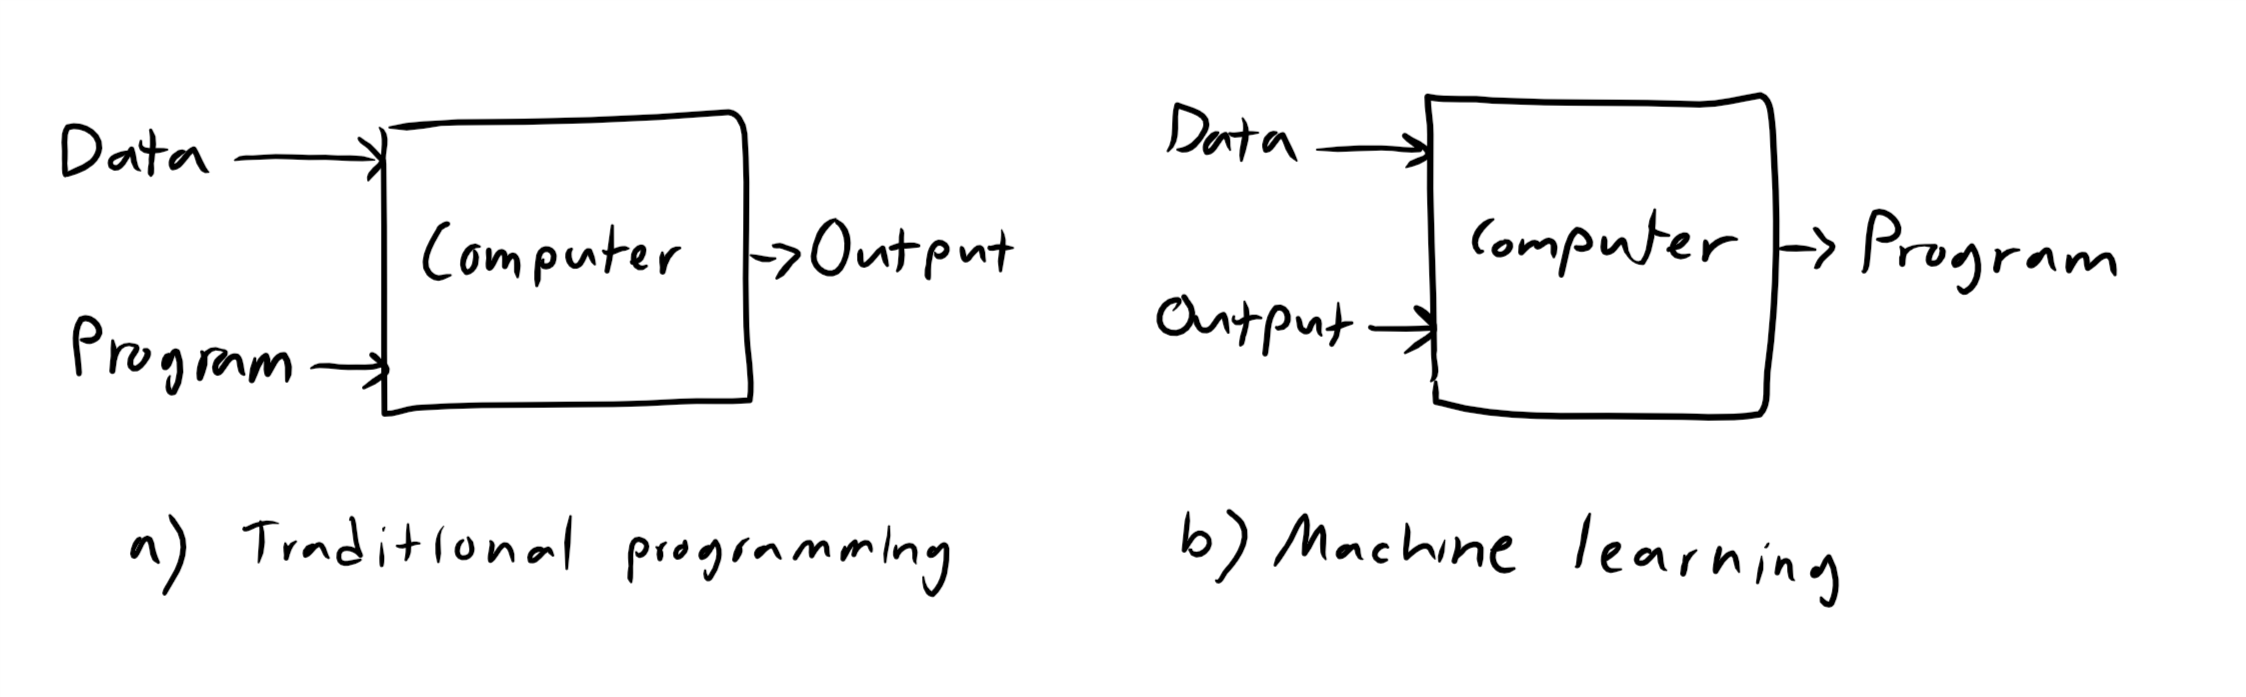
\includegraphics[width=0.9\linewidth]{gfx/figures/traditionalvsml.png}
\caption{''Traditional'' programming and machine learning}
\label{fig:traditionalvsml}
\end{figure}

In classification tasks the models try to predict a \emph{class} for an unknown datapoint. The classes are discrete and the number of classes is finite. In binary classification there are two possible classes, often labelled 1 and 0, or true and false, as seen in the email example above. In regression tasks the predictions result in a real number instead of discrete values, such as when predicting a length of time.
Different models are used for these different tasks.
The model best suited for an application depends on the distrubution of the possible values and other characteristics of the phenomenom being modeled.

In conclusion, Machine Learning is a set of algorithms and models that leverage a large dataset to estimate some feature of new datapoints.
In classification tasks, this feature is chosen from a finite set of possible classes, whereas in regression tasks the value estimated is a real number.

\subsubsection{Regression}

Regression algorithms use a set of training data to learn a model.
The training data consists of a large set of labelled data points.
The data set is often large, consisting of thousands of data points.
Each data point consists of a set of \emph{features} (the inputs) and a \emph{label} (the output).
The features are some aspects of the data point that are always available or can be measured.
The label is the feature that is unknown and we want to estimate for new data.

For example, regression could be used to estimate wine quality.
The features could be some measurable aspects of the wine such as the pH-value, the amount of sugar, or the year bottled.
The label would be a number ranging from 1 to 10 corresponding to the quality of the wine.
A data set could be generated by measuring the features of many wines and then having human wine tasters manually label them with their understanding of the wine quality.
This set of features and labels could then be used to train a regression model.
The model could then be used to estimate the quality of a previously unseen wine by measuring the same features and inputting them to the model.
The model would then output a number from 1 to 10 as the estimate for the wine quality.

Expressed mathematically, regression estimates an output value $r \in \mathbb{R}$, which is a real number \cite{alpaydin}.
The training set consists of $N \in \mathbb{N}$ feature vectors (inputs) $\mathbf{x}^t \in \mathbb{R}^d$ and $N$ output values $r^t$.
Here $d \in \mathbb{N}$ is the number of features used as inputs.
$$\mathcal{D} = \{(\mathbf{x}^t, r^t)\}_{t=1}^N, \mathbf{x}^t \in \mathbb{R}^d, r^t \in \mathbb{R}$$
The regression algorithm (the learner) processes the training data and outputs a model $g(\mathbf{x})$ which estimates the output parameter $r$ for a new unseen feature vector $\mathbf{x} \in \mathbb{R}^d$.
$$g(\mathbf{x}) = r$$

The model $g(\mathbf{x})$ is chosen based on the data and domain knowledge. 
The models can range from a simple linear models to complex models such as decision forests.
In theory any model $g: \mathbb{R}^d \rightarrow \mathbb{R}$ can work,
as long as a learning algorithm for the model exists.
In the case of features that are not real numbers, a mapping function is used that takes a different type of feature (such as a string or a boolean) and converts it into a real number.
In the ideal case the model should fit the phenomenon (physical or other) being modeled in the machine learning application.
However, sometimes the underlying model is not known. 
In these cases multiple models can be used and compared based on the dataset and any information is available.

The model is evaluated over a separate test set.
Commonly, the test set is created by separating the training set into two distict sets before the training phase.
$$\mathcal{D}_{test} = \{ (\mathbf{x}_*^t , r_*^t) \}_{t=1}^{N_{test}}$$
A metric such as the \emph{mean square error} (MSE) can be used as a score to evaluate the model. \cite{alpaydin}
$$E(g | \mathcal{D}_{test}) = \frac{1}{N_{test}} \sum_{t=1}^{N_{test}} (r_*^t - g(\mathbf{x}_*^t))^2$$
In essence, the model is tested with the inputs of a data point in the test set. The output value from the model is compared to the ''correct'' label in the test set data point.
The difference between the values is the \emph{error}.
The aim of machine learning is to minimize this error by choosing a good model for the application and the data, and tuning the model parameters until the desired (low) error is reached.

All this is based on the assumption that the samples are \textit{independent and identically distributed} (iid) \cite{alpaydin}.
This means that the order of the samples in the sets does not matter and that the distribution of the features and the labels is the same in the training set, the test set, and for any unseen data point outside these sets.
If there is enough information in the training set, the model should be able to use the information to label new data points with the same performance as over the test set.
Thus, the performance over the test set can be used to estimate the performance of the model for unseen data.

There are many different regression learners that are based on different theories. The two models used in this thesis are Poisson Regression \cite{azurepoisson} and Boosted Decision Trees \cite{azurebdt}.

\subsubsection{Poisson regression}

Poisson regression models data with labels that fall into a poisson distribution.
Poisson distribution often describes count data, such as the count or probablility of events happening during a fixed time interval. \cite{osgood2000poisson}
When graphed, the distribution has a peak in the beginning and long tail, as seen from figure \ref{fig:poissongraphs}.

\begin{figure}[htb]
\centering 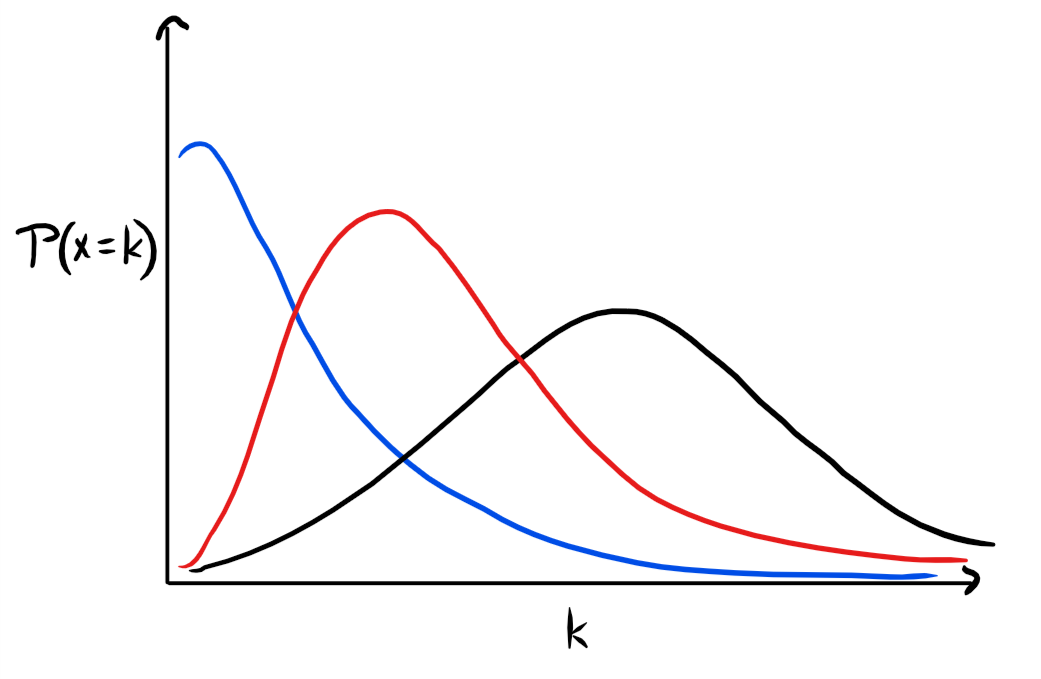
\includegraphics[width=0.6\linewidth]{gfx/figures/poissongraphs.png}
\caption{Poisson distributions with different expected values of $k$}
\label{fig:poissongraphs}
\end{figure}

\nyi{Explain more theory? (mathematics)}

% Talk about practical usage (strengths, limitations)
A poisson regression model works well in data involving counts and times that are distibuted along a poisson distribution. 
In other types of data the poisson regression model will not give good results.

\subsubsection{Boosted decision trees}

The second model used in this thesis is boosted decision trees (BDT).
A \textit{decision tree} is a model for supervised learning that is based on a sequence of splits \cite{alpaydin}.
The splits form a hierarchical tree.
The tree consists of internal decision nodes and the terminal leaves containing values.
To find the result of the regression model, the algorithm steps through the decision nodes starting from the root.
At each node a component of the feature vector is compared against a predetermined threshold value.
If the value is lower (or higher) than the threshold value, a decision is made and either the left or the right child node is chosen.
This is repeated until a terminal leaf node is reached at the bottom of the tree. 
The terminal nodes contain the label values.
The value in the leaf reached by the iterative algorithm is the result of the regression model.

The boosted decision tree learner in Azure ML is based on LambdaMART \cite{azurebdt}.
LambdaMART is a set of algorithms that implement a \textit{forest} of regression trees \cite{lambdamart2010}.
Gradient boosting \cite{friedman2001greedy} is used to build a model combining several weaker models to form a stronger model.
The forest consists of multiple decision trees.
The result of the regression given by the LambdaMART forest is a linear combination of the outputs of the trees.
The learner trains the thresholds at the decision nodes and the values at the terminal leaves of each tree, as well as the weights for the linear combination to minimize error over the training set.

\nyi{Write above paragraph with mathy expressions?}

% Talk about practical usage (strengths, limitations)
One strength of the boosted decision tree model is that it is highly interpretable and can be used for rule extraction \cite{alpaydin}. Each tree can be converted into a set of IF-THEN rules, and the weights of the linear combination correspond to the importance of each tree. 
Because of these reasons, the domain expert can analyze the model to see which features are being used and whether the model seems to make sense.
Furthermore, the model can even provide information about the real world ruleset for the measured phenomenon.
In general, boosted decision trees work well when the components of the feature vectors are related. In the case of completely independent vectors, a BDT model will not be as good \cite{azurebdt}.

%%%%%%%%%%%%%%%%%%%%%%%%%%%%%%%%%%%%%%%%%%%%%%%%%%%%%%%%%%%%%%%%%%%%%%%%%%%%%%%%
%%% Related work
%%%%%%%%%%%%%%%%%%%%%%%%%%%%%%%%%%%%%%%%%%%%%%%%%%%%%%%%%%%%%%%%%%%%%%%%%%%%%%%%

%\clearpage
\subsection{Related work}
\label{sec:relatedwork}

Process mining has gained interest in the recent years, since it offers possibilities of streamlining business processes and gaining business intelligence (BI) by finding bottlenecks and inefficiencies in the processes.
Process mining has many uses, such as process discovery \cite{van2016discovery, van2013discovering}, trace clustering \cite{de2016general}, and conformance checking \cite{chomyat2016process}. Furthermore, there's some research done in the area of automatically detecting process anomalies automatically \cite{bezerra2009anomaly}.

Process discovery is in the heart of process mining, since most process mining methods rely on modeling the process and taking advantage of the model in some manner.
Because of this, process discovery is talked about in many papers related to process mining \cite{chomyat2016process, de2016general, van2013discovering, van2015extracting, van2016process,bezerra2009anomaly}.

Conformance checking means making sure the current process conforms to a previously determined set of rules or a model \cite{chomyat2016process}.
Conformance checking can be especially useful in sectors where conforming to regulations or other such rules is critical for the work.
Examples of such sectors are the financial sector, medical business, and government institutions.
Process mining can be used to ensure the regulations are being followed.

The main purpose of my thesis is to help visualize the processes and to show anomalies to the users or even notify about them automatically.
The definition of \textit{anomaly} is not consistent across research \cite{bezerra2009anomaly}. 
An anomaly can be anything exceptional or abnormal in the behaviour of a system. 
It can also describe an error, noise, or fraudulent behaviour.
Usual definitions include that an anomaly needs to be infrequent, unexpected, and something that deviates with the normal behaviour.
Precise definition is difficult to formally define, since the definition of what is considered ''normal'' differs between cases. 
Bezerra et al. \cite{bezerra2009anomaly} present how an established process mining tool ProM can be used to discover models and check their conformance.
Each trace gets assigned a conformance value (fitness) describing how well it fits the previously discovered model.
With this method, a threshold value for required model fitness can be assigned to find the anomalous traces.
However, there is little focus on detecting anomalies real-time.

The past event logs can also be used to build workload histograms \cite{getta2014mining}.
This method reads event logs with periodic patterns (such as the re-occuring submissions in the Microsoft store).
The workload information can be used to predict incoming workloads to improve system performance by preparing against peak loads.
This method is \textit{process enhancement}. 
An example of process enhancement is detecting periods of low activity and using them to run background tasks.
This type of balancing decreases the idle time of a system and improves its capability to respond to peak loads \cite{getta2014mining}.

\nyi{highlight the lack of real-time somewhere?}